
\documentclass[envcountsame]{llncs}
\usepackage{amsmath}
\usepackage{amsfonts}
\usepackage{graphicx}
\usepackage{subfigure}
\usepackage[linesnumbered,boxed]{algorithm2e}

\setlength{\abovecaptionskip}{10pt} 
\setlength{\belowcaptionskip}{-10pt}


\begin{document}
\title{Realtime Event Summarization from Tweets with Inconsistency Detection}
\author{Lingting Lin, Yunjie Wang, Chen Lin}
\institute{Department of Computer Science, Xiamen University \email{chenlin@xmu.edu.cn}}

\maketitle
\begin{abstract}
The overwhelming amount of event relevant tweets highlights the importance of realtime event summarization systems. Previous studies couldn't guarantee the integrity of a realtime summary. When new information emerges, the former summary should be updated accordingly to deliver most recent, authoritative, and correct information. For example, when the number of injuries increases in an Earthquake, the old number in the former summary must be replaced to avoid inconsistency of the summary. In this contribution we present a realtime event summarization system with explicit inconsistency detection. We model the realtime summarization problem as integer programming problems and solve the relaxed linear programming form by simplex method. To reduce the storage and computation cost of expensive inconsistency detection, we embed a fast inconsistency detection strategy in the simplex algorithm. Experiments on real twitter sets demonstrate the efficiency and effectiveness of our method. 
\end{abstract}
\section{Introduction}
%Motivation
Accidents, disasters, political rallies...we are eager to gather information about different kinds of live events that happen around us. In the past, we rely on experienced journalists to cover the stories. At now, thanks to the large community of micro-blogging users, we are provided with instant reports published by individuals and organizations all over the world.  More and more people today rely on microblogging contents, such as Tweets, to seek information about live events. However, the huge volume of event related tweets could be overwhelming. For example, TweeStudy shows that the majority (over $85\%$) of trending topics in microblog sphere are headline news and real-life events~\cite{kwak2010twitter}. An event summarization system is needed to facilitate knowledge management and improve user experiences.

We have witnessed rapidly increasing popularity of research efforts in event summarization from tweets~\cite{Takamura2011Summarizing,Lin2012Generating,Rudra2015Extracting,Shou2013Sumblr,Liu2016LEDS,Gillani2017Post,Zubiaga2012Towards,Sharifi2010Summarizing}.   Most previous work are based on extractive method, i.e. they extract a smallest set of representative tweet reports to form a brief summary. Extractive methods are easy to implement and have shown to perform well~\cite{Takamura2011Summarizing,Lin2012Generating,Rudra2015Extracting,Shou2013Sumblr,Liu2016LEDS,Gillani2017Post,Zubiaga2012Towards}. Our arguments are founded on extractive summarization methods.

%requirement: realtime
Beyond the usual requirements for text summarization systems, such as coverage and representativeness of the summary,  event summary must also be \textbf{realtime}. On one hand, the response must be fast. The summary must be efficiently updated as new tweets arrive. On the other hand, the summary must report the current status of the event. As an ongoing event often involves changing information, report must be updated to include new information when it emerges.

%inconsistency
During the update process, the integrity of the summary must be preserved.  An outdated report must be replaced if it leads to \textbf{inconsistency} in the summary. An inconsistent summary is harmful for most live events because it is confusing and misleading. In particular, for natural disaster or group incidents,  users are interested on  information such as number of injuries, suspects description and so on. We here list three scenarios when a former report needs to be replaced because of inconsistency. (1) The information changes as a natural consequence of event evolution. For example, in an earthquake the number of injuries is increasing over time. Thus the numbers in previous summaries become obsolete and they should be replaced by the most up-to-date numbers. (2) Multiple information sources provide conflicting information. For example, the number of injuries is often estimated by several parties, such as  bystanders, hospitals and so on. When a more authoritative source, such as the local government announces the new estimate, the old estimates in previous summaries are no longer credible and must be replaced. (3) The information in previous summaries is wrong. For example, the police have suspected the wrong person and now they update the description. In this case, the realtime event summarization system must select the correct tweet to replace former reports.


%open problem: no related work prevent inconsistency in
Realtime event summarization from Tweets is still an open problem. In the literature, most of previous works treat the problem as producing different forms of summaries from a static set of tweets~\cite{Takamura2011Summarizing,Lin2012Generating,Rudra2015Extracting,Liu2016LEDS,Gillani2017Post}. A few recent research works focused on efficient algorithms to summarize the tweet streams~\cite{Shou2013Sumblr,Zubiaga2012Towards}. Their summarization systems are based on coarse grained semantic analysis, and thus are not able to detect inconsistency. Though we have shown that integrity of the event summary is crucial, to the best of our knowledge, none of the previous works is able to produce a realtime event summarization which is guaranteed to exclude inconsistent information.


%challenge
Two challenges arise in producing realtime event summarization without inconsistent information.

%Algorithm
The first challenge lies in the macro-level algorithm. Realtime summarization requires an efficient algorithm to analyze the streaming tweets. As the amount of available tweets constantly increases to infinity, re-computation based on a complete set of all tweets up to the current timestamp is infeasible. The ideal algorithm is to  incorporate new tweets as they become available, and discard old tweets when possible to limit the storage and speed up processing.

%inconsistency detection
The second challenge is related to the micro-level analysis to detect inconsistency. Inconsistency detection is based on pair-wise similarity. Coarse grained semantic analysis, such as the cosine similarity measure based on the bag of words representation in previous works~\cite{Takamura2011Summarizing,Lin2012Generating,Rudra2015Extracting,Shou2013Sumblr,Liu2016LEDS,Gillani2017Post,Zubiaga2012Towards,Sharifi2010Summarizing} is suitable to capture topic similarity in a summarization, but is not able to detect inconsistent information. Inconsistency is revealed via word order and syntactic structures. We need to assess information similarity based on the combination of semantic, lexical and syntactic analysis. Furthermore, inconsistency detection is computationally expensive. It is important to avoid unnecessary pair-wise comparisons.

%idea: micro level:
Our goal in this paper is to design a system that delivers realtime summary with integrity from tweets. To address the first challenge, we assume that, the realtime summarization problem given a small batch of new tweets can be modeled as two integer programming problems, one of which on the old tweets, and another on the new batch. Both integer programming problems can be relaxed to linear programming problems and be solved by the simplex method. In each update we first optimize the problem on the new batch. We use the solution on the new batch to modify the problem on the old tweets and incrementally update the summary.  In this manner, we do not need to store or operate on the complete tweet set and the full similarity matrix.


To address the second challenge, we propose skeleton similarity: a new similarity metric to assess information similarity between any pair of tweets. An inconsistency detection strategy, which is a combination of the skeleton similarity and authority estimation heuristics, is then adopted in the pivoting operation in the simplex method. It has two advantages in embedding the skeleton similarity computation in the simplex algorithm. (1) It significantly reduces the number of information similarity comparisons. (2) It ensures that the former summary will be replaced by most up-to-date, authoritative and correct information.


%contributions
Our contributions are three folds. (1) The integrity of event summary is a relatively unexplored area in Tweet summarization. We propose to improve the integrity of event summarization by explicit inconsistency detection. (2) Our system is targeted towards text streams. We model the realtime summarization problem as integer programming problems in small batches. We differ from existing work in that we enable incremental update in the simplex method framework. (3) We propose a novel skeleton similarity to efficiently and effectively capture inconsistency.

%paper structure
This paper is organized as follows. We briefly survey the related work in Sec.~\ref{sec:related}. In Sec.~\ref{sec:static}, we first introduce the idea of modeling a summarization problem as an integer programming problem and the standard simplex procedure to solve the relaxed linear programming problem. In Sec.~\ref{sec:dynamic}, we give the problem definition for realtime event summarization given a small batch of new tweets and the improved simplex solution. The inconsistency detection strategy is a component of the simplex update algorithm. We present and analyze the experimental results on a real data set in Sec.~\ref{sec:experiment}. We conclude our work and suggest future directions in Sec.~\ref{sec:conclusion}.

\section{Related Work}\label{sec:related}
%Tweet summarization belongs to the more general category of multi-document summarization. We start by reviewing the common approaches in multi-document summarization. Then we move on to describe the recent research trend of tweet summarization.

%\subsection{Multi-document Summarization}
%first paragraph: multi document summarization
%??LPR, SNMF??
Multi-document summarization conveys the main and most important meaning of several documents. There are generally two types of summarization techniques. One type is extraction-based summarization, which extracts objects from the entire collection and combines the objects into a summary without modifying the objects themselves. The other type is abstraction-based summarization which rephrases the source document. The majority of summarization systems are extractive. The extracted objects are often sentences. The selection is usually based on the representativeness of sentences, i.e. with significant frequency~\cite{Yih2007Multi-document}, or is a structural centroid in a sentence graph~\cite{Lin2012Generating}, or is considered important by a submodularity function~\cite{MSSF}. 

%second paragraph: event summarization 
%Recently, a number of studies devote to summarizing documents related to events, mostly news articles. In~\cite{Lin2008Storyline-based} a main theme is extracted by selecting representative sentences in each time segment of the event. ETS~\cite{Wang2009Evolutionary} returns the evolution skeleton along the timeline by extracting representative and discriminative sentences at each phase. In~\cite{Yan2011Evolutionary} representative sentences are chosen based on relevance, coverage, coherence and cross-date diversity.


%\subsection{Tweet Summarization}
%first paragraph: tweet summarization
The emergence of Twitter motivates recent research works on summarizing microblogging contents. Tweet summarization systems are successfully applied in entity-centric opinion summarization~\cite{Meng2012Entitycentric}, personal summarization of interesting content~\cite{Ren2013Personalized,Chin2017TOTEM}, search results grouping \cite{Mathioudakis2010TwitterMonitor}, and summarizing tweets for natural or social events~\cite{Takamura2011Summarizing,Lin2012Generating,Rudra2015Extracting,Shou2013Sumblr,Liu2016LEDS,Gillani2017Post,Zubiaga2012Towards}.

%realtime
At the algorithm level, tweet summarization also use extractive and abstractive methods. Except a few works which are based on abstractive method~\cite{Sharifi2010Summarizing}, most tweet summarization methods rank and select the most representative tweets. A few recent works start to improve general multi-document summarization methods for better efficiency. In~\cite{Shou2013Sumblr}, an incremental clustering method is presented. In ~\cite{Zubiaga2012Towards} the selection range is shrinked by detecting sub-events and selecting one sentence with maximal similarity to any new sub event.

% inconsistency
To achieve a better performance, the noisy and social nature of microblogs must be taken into consideration. Most tweet summarization systems will identify influential tweets~\cite{Hannon2010Recommending},  promote most recent tweet~\cite{Efron2011Estimation}, and circumnavigate spam and conversational posts~\cite{Gillani2017Post}. However, the integrity of summary has not yet been fully studied. The work that is most related to ours is the 
classification and summarization of situational information in~\cite{Rudra2015Extracting,Rudra2016Summarizing}. However they do not explicitly identify inconsistency as they simply provide all versions of inconsistent information. And they do not accelerate algorithms for realtime response. 


\section{Static Summarization}\label{sec:static}
%
The standard summarization task is conducted on a static set of tweets. We refer this task as a static summarization. In this section, we first model the static summarization problem as an integer programming problem. We then present a high level explanation about the simplex method. We finally give an outline for the algorithm to solve static summarization.
\subsection{Problem Definition}
%prelimiraries
Suppose that we have a universe of $N$ \emph{candidate} tweets, within which $M$ tweets are credible and relevant. The credible and relevant tweets are important so they are considered to be the \emph{seeds} of the summary. The extractive method for any static summarization is to select a few representative tweet \emph{reports}\footnote{To distinguish the three types of tweets, we will refer the tweets to be summarized as candidates, the tweets in the summary as reports, and the credible and relevant tweets as seeds.} from the tweet universe to form the summary. To model this problem, we use a vector $\mathbf{x}\in \mathcal{R}^N$ , where each element $\mathbf{x}_j\in \{0,1\}$ is a binary variable. If a candidate  $i$ is chosen to be a report in the summary, the corresponding $x_i=1$ . Otherwise, we set  $x_i=0$. We use another $N$-dimensional vector $\mathbf{c}\in \mathcal{R}^M$ to describe the loss of choosing each candidate as a report. $\mathbf{A}\in\mathcal{R}^{M\times N}$  is a similarity matrix, where $A_{i,j}$  is the similarity between a seed $i$ and a candidate $j$ in the tweet universe. $\mathbf{b}\in \mathcal{R}^{M}$ is a weight vector, where $b_{i}>0$ indicates the importance of seed $i$ being covered in the summary. Our objective is to

\begin{equation}\label{equ:integerstatic}
\min \mathbf{c}^T \mathbf{x} \textrm{ subject to } \mathbf{A} \mathbf{x} \geq \mathbf{b}, \forall i\textrm{ } x_i\in \{0,1\}.
\end{equation}

The optimization problem in Equ.~\ref{equ:integerstatic} aims to find a minimal set of reports that deliver all credible and relevant information. Thus the result summary achieves brevity, coverage and representativeness. The decision of $b,c$ and the $M$ indices affects the performance of summarization. We allow the flexibility of choosing any sounding technique to determine the credible and relevant set of tweets, their importance value and the loss of choosing any candidate. In this work,  we  choose the top $M$ results from a search engine, determine $\mathbf{b}$  by estimating  the authority of each tweet account, and assign $\mathbf{c}$ by assessing the textual quality of each candidate. The technical details will be discussed in Sec.~\ref{sec:experiment}.

\subsection{The Simplex Method}
We transform the integer programming problem in Equ.~\ref{equ:integerstatic} to a bounded linear programming problem by making the following adjustments: $\tilde{\mathbf{c}}=[\mathbf{c},\mathbf{0}],\tilde{\mathbf{x}}=[\mathbf{x},\mathbf{z}]^T,\tilde{\mathbf{A}}=[\mathbf{A},-\mathbf{I}]$, where $\mathbf{z}\in\mathcal{R}^M$, $ \mathbf{I}$ is the $M\times M$ identity matrix. Therefore we have the following objective

\begin{equation}\label{equ:linear}
\min \tilde{\mathbf{c}}\tilde{\mathbf{x}}\textrm{ subject to } \tilde{\mathbf{A}}\tilde{\mathbf{x}} = \mathbf{b}, \forall 1\leq j\leq N,\textrm{ } \tilde{x}_j \leq 1, ,\tilde{\mathbf{x}}\geq \mathbf{0}.
\end{equation}

The linear programming problem in Equ.~\ref{equ:linear} can be solved by the simplex method. Each iterate in the simplex method is a \emph{basic feasible point} that (1) it satisfies $\tilde{\mathbf{A}}\tilde{\mathbf{x}} = \mathbf{b}, \forall 1\leq i\leq M+N,\tilde{x}_i \geq 0,\forall 1\leq j\leq N, \tilde{x}_j \leq 1$ and (2) there exists three subsets $\mathcal{B,U.L}$ of the index set $\mathcal{A}=\{1,2,\cdots M+N\}$ such that $\mathcal{B}$ contains exactly $M$ indices, $\mathcal{A}=\mathcal{B}\cup \mathcal{U} \cup \mathcal{L}$ and $i \in \mathcal{U} \Rightarrow \tilde{x}_i=1,i \in \mathcal{L} \Rightarrow \tilde{x}_i=0$.

The major issue at each simplex iteration is to decide which index to be removed from the basis $\mathcal{B}$ and replaced by another index outside the basis $\mathcal{B}$.  As the optimal is achieved when the KKT conditions are satisfied, in each simplex iteration first  a \textbf{pricing} step is conducted to check on the KKT conditions.  If the KKT conditions are satisfied then the problem is solved. Otherwise a \textbf{pivoting} operation is implemented to select entering and leaving indices.

%We should keep in mind that the simplex iterations are run on basic feasible points. 
To obtain an easy start of basic feasible points, we solve the following linear programming problem.

\begin{equation}\label{equ:linearphaseI}
\min \mathbf{e^{T}s} \textrm{ subject to } \tilde{\mathbf{A}}\tilde{\mathbf{x}} + \mathbf{Is} = \mathbf{b},  \forall 1\leq j\leq N,\textrm{ } \tilde{x}_j \leq 1, ,\tilde{\mathbf{x}}\geq \mathbf{0}, \mathbf{s}\geq \mathbf{0},
\end{equation}

where $\mathbf{e}$ is the vector of all ones, $\mathbf{I}$ is a diagonal matrix whose diagonal elements are $I_{ij}=1$. $\mathbf{s}$ are called artificial variables. It is easy to see that the solution to Equ.~\ref{equ:linearphaseI} is a basic feasible point for Equ.~\ref{equ:linear}, if the objective $\mathbf{e^{T}s}=0 $.

The remaining problem is that the solution we obtained for Equ.~\ref{equ:linear} are not integers. As our interest is on the variables $\mathbf{x}$ in Equ.~\ref{equ:integerstatic}, we can intepretate the values obtained for Equ.~\ref{equ:linear} $\tilde{x}_j, \forall 1\leq j\leq N $ as the probability of choosing $j$ as a response. For indices that are in the upper bound set $j \in \mathcal{U}$, the corresponding candidate is deemed in the summary. For indices that are in the lower bound set $j \in \mathcal{L}$, the corresponding candidate is filtered. For the remaining candidates, we perform a \textbf{rounding} algorithm. We first sort the solution we obtained for Equ.~\ref{equ:linear} in descending order of its values $0< \tilde{x}_j< 1,\forall 1\leq j\leq N$ and then sample $x_j$ based on the probability of assigned value $\tilde{x}_j$. 

\begin{equation}
p(x_j=1)= \tilde{x}_j, \forall 1\leq j \leq N
\end{equation}



To conclude this section, we present Algorithm.~\ref{alg:framework}. The frameowk of static summarization includes three steps. The first stage (step 1 to step 2) is to obtain a basic feasible point for the linear programming problem Equ.~\ref{equ:linear}, the second stage (step 3 to step 4) is to optimize the linear programing problem in Equ.~\ref{equ:linear}, and the third stage (step 5) is to obtain the integer solutions for Equ.~\ref{equ:integerstatic}.   

\begin{algorithm}\label{alg:framework}
\caption{The framework for static summarization}
\KwIn{$\mathbf{c,b}, A$}
\KwOut{$\mathbf{x}$}

Initialize $\tilde{\mathbf{x}}=\mathbf{0},\tilde{\mathbf{A}}=[\mathbf{A},-\mathbf{I}],\mathbf{s}=\mathbf{b}$\;
Solve $\min \mathbf{e^{T}s} \textrm{ subject to } \tilde{\mathbf{A}}\tilde{\mathbf{x}} + \mathbf{Is} = \mathbf{b},  \forall 1\leq j\leq N,\textrm{ } \tilde{x}_j \leq 1, ,\tilde{\mathbf{x}}\geq \mathbf{0}, \mathbf{s}\geq \mathbf{0}$ by simplex method\;
Initialize $\tilde{\mathbf{x}}$ by the solution above, set $\tilde{\mathbf{c}}=[\mathbf{c},\mathbf{0}]$  \;
Solve $\min \tilde{\mathbf{c}}\tilde{\mathbf{x}}\textrm{ subject to } \tilde{\mathbf{A}}\tilde{\mathbf{x}} = \mathbf{b}, \forall 1\leq j\leq N,\textrm{ } \tilde{x}_j \leq 1, ,\tilde{\mathbf{x}}\geq \mathbf{0}$ by simplex method\;
$\tilde{\mathbf{x}}=[\mathbf{x},\mathbf{z}]^T,$ Rounding $\mathbf{x}$\;
%delete?
\end{algorithm}



\section{Dynamic Summarization}\label{sec:dynamic}
For streaming text, the realtime summarization system must be able to update the summary as new contents arrive. The summary is dynamic because it changes over time. We here consider a batch setting: the summary is updated when a predefined number $T$ of tweets are received. Note that if we set $T=1$ we enable online update.  In this section, we first model the dynamic summarization problem and then we present the improved simplex method.

\subsection{Problem Definition}
%candidate universe
When a small batch of tweets arrive, the candidate universe will be a new set of $N_1 $ candidates with importance weights denoted by $\mathbf{c_1}$ and the former candidates. We only keep previous reports $\mathbf{x_0}$ with $x_i=1$ in the former summary and their loss value $\mathbf{c_0}$  and discard everything else from former corpus to reduce storage space.

%b
To produce a summary that covers the demanded information, the model in Sec.~\ref{sec:static} requires a predefined set of credible and relevant seed tweets and their importance weights $\mathbf{b}$. It is crucial here to mention that in the dynamic setting the seed set is priorly unknown due to inconsistency. For example, if a new credible tweet is found to conflict with a former credible tweet, then the former one must be excluded. Suppose we have $M$ seeds, but the integrity is not guaranteed. It is possible to check on inconsistency to prune the $M$ seeds to identify a consistent new set. However, the inconsistency detection algorithm on $M\times (M-1)$ pairs is expensive. Henceforth, our idea is to call the inconsistency detection algorithm only when it is necessary. 

%assumption
Suppose we segment the timeline of tweets into two divisions. $M_0$ represents the set of seeds that are covered by the former summary, $M_1$ is the set of seeds published after the former summary was generated. $M_1$ is generated as follows. We first retrieve $R$ relevant tweets published after the summary. Then we can adopt any heuristic to fast prune inconsistent seeds in $M_1$. We can also adopt any external strategy to exclude seeds that are less credible than any seed in $M_0$. Therefore the seeds in $M_1$ must be covered with priority if they are inconsistent with the seeds in $M_0$, because any seed in  $M_0$ is newer and at least as credible as any seed in $M_1$.  To deliver an up-to-date summary, we set $\mathbf{c}$ so that the loss for new candidates is smaller than the old candidates.




%model two phases
Below we give the architecture of the dynamic summarization system. We model the dynamic summarization as sequential integer programing problems.  Given the whole set of candidates $\mathbf{x_0,x_n}$ and the associated loss $\mathbf{c_0,c_n}$, the importance of possible seeds $\mathbf{b_1}$, at stage I, we first solve the optimization problem for the higher division of seeds. 

\begin{equation}\label{equ:stageI}
\min \mathbf{c_0}^T \mathbf{x_0} + \mathbf{c_1}^T \mathbf{x_1} \textrm{ subject to } S \mathbf{x_0} + B\mathbf{x_1} \geq \mathbf{b_1}, \forall i, \forall j\in \{0,1\}\textrm{ } x_{j,i}\in \{0,1\}.
\end{equation}

In solving Equ.~\ref{equ:stageI} we will obtain the refined seed set $\mathbf{b_0}$. In stage II we solve the optimization problem:
\begin{eqnarray}
\min \mathbf{c_0}^T \mathbf{x_0}+\mathbf{c_1}^T\mathbf{x_1}\\\nonumber
s.t. \begin{bmatrix}
F & D \\
S & B
\end{bmatrix}\begin{bmatrix}
 \mathbf{x_0}\\
\mathbf{x_1}
\end{bmatrix}\geq \begin{bmatrix}
\mathbf{b_0}\\
\mathbf{b_1}
\end{bmatrix},\\\nonumber
 \forall i, \forall j\in \{0,1\}\textrm{ } x_{j,i}\in \{0,1\}, 
\end{eqnarray}

where $F\in \mathcal{R}^{M_0\times N_0}$ is the similarity matrix between former reports and old tweets, $D\in \mathcal{R}^{M_0\times N_1}$ is the similarity matrix between new candidates and old credible tweets, $S\in \mathcal{R}^{M_1\times N_0}$ is the similarity matrix between old reports and new credible tweets, $B\in \mathcal{R}^{M_1 \times N_1}$ is the similarity matrix between new candidates and new credible tweets.

%algorithm overview
\subsection{Simplex Update Method}

%initialization
As in Sec.~\ref{sec:static}, we introduce new variables.  $\tilde{\mathbf{c}}=[\mathbf{c_0},\mathbf{c_1}, \mathbf{0}],\tilde{\mathbf{x}}=[\mathbf{x_0},\mathbf{x_1},\mathbf{z}]^T,\tilde{\mathbf{A}}=[F,B,-\mathbf{I}],\mathbf{s}$, where $\mathbf{z}\in\mathcal{R}^{M_1}$, $ \mathbf{I}$ is the $M_1\times M_1$ identity matrix. To initialize, we set  $\mathbf{x_0}=\mathbf{1}$ and keep $\mathbf{x_0}$ fixed while solving Equ.~\ref{equ:linearphaseI}. We use the solution as the initialized guess for the second stage optimization. 

%pricing
In each iterate of simplex, we first operate the pricing step.  Let's compute $\bar{c_j} = c_j - y^T\mathbf{A}_{,j}^{'}$ for every $\tilde{x_j}$ not in the basis, where $\mathbf{y} = {\mathbf{B}^T}^{-1}\mathbf{c_B}$,. If $\tilde{x_j }= 0, \bar{c_j} > 0$ and $\tilde{x_j} = 1,\bar{c_j} < 0$, then the objective function is optimized. Otherwise we implement the pivoting operation.


%pivoting
We modify the conventional pivoting operation in the simplex method. In the initialization we keep $\mathbf{x_0}=\mathbf{1}$, which indicates that the constraint is satisfied with all the former reports kept. If the pricing step suggests the objective function is not optimized, there are usually multiple indices which violate the KKT conditions.  Hence in selecting the entering index, we prefer a $z$ index, because selecting an auxiliary variable leads to minimal modification of the summary. However, if an index from $\mathbf{x_0}$ is to leave and an index from $\mathbf{x_1}$ is to enter, a new tweet is able to cover the same set of seeds with smaller cost (given that we assign higher loss $c_0$ to old tweets). We can not rule out the possibility of inconsistency. In fact, inconsistency only happens when two tweets are semantically closely related. Therefore we conduct inconsistency test between the entering index and the leaving index. If the leaving index is found to be inconsistent of the new report, we delete the corresponding component $x_{0,i}$ from the problem. This strategy ensures that inconsistent candidates do not repeatedly enter and leave the summary. We remove all seeds that are related to $x_{0,i}$ in $\mathbf{b_0}$. The pivoting operation is described in Algorithm.~\ref{alg:pivoting}.

%


\begin{algorithm}[ht]\label{alg:pivoting}
\caption{Pivoting in the simplex update method}
    $q = \arg\max_{j} \left\{10\times\bar{c_j}\textrm{ } \forall j\in \mathbf{z_N}, \bar{c_j} \textrm{ } \forall j\in\{\mathbf{x_L}  \},-\bar{c_j}\textrm{ }  \forall j\in\mathbf{x_U}  \right\}$\;
    $d = \mathbf{B}^{-1}\mathbf{A}_{,q}^{'}$\;
    \If{$q \in \{ \mathbf{z_N}\}$}
    {
        $x_q^{new} = \min_i \left\{\{\frac{x_{\mathbf{B}_{i}}}{d_i}, \frac{s_{\mathbf{B}_{i}}}{d_i}, \frac{z_{\mathbf{B}_{i}}}{d_i}\} \forall d_i>0,\{\frac{x_{\mathbf{B}_{i}}-1}{d_i}\} \forall d_i<0\right\}$\;
        $\mathbf{x}_{\mathbf{B}^{old}}^{'new} = \mathbf{x}_{\mathbf{B}^{old}}^{'old} - dx_q^{new}$\;
        $p=\arg\min_{i}$\;

    }
    \If{$q \in \mathbf{x_L}$}
    {
        $x_q^{new} = \min_i \left\{\{\frac{x_{\mathbf{B}_{i}}}{d_i}, \frac{s_{\mathbf{B}_{i}}}{d_i}, \frac{z_{\mathbf{B}_{i}}}{d_i}\} \forall d_i>0, \{\frac{x_{\mathbf{B}_{i}}-1}{d_i}\} \forall d_i<0, 1 \right\}$\;
        $\mathbf{x}_{\mathbf{B}^{old}}^{'new} = \mathbf{x}_{\mathbf{B}^{old}}^{'old} - dx_q^{new}$\; \If{$x_q^{new} \neq 1$}
        {
            $p=\arg\min_{i}$\;
        }
    }
    \If{$q \in \mathbf{x_U}$}
    {
        $x_q^{new} = 1 - \min_i \left\{\{\frac{x_{\mathbf{B}_{i}}}{-d_i}, \frac{s_{\mathbf{B}_{i}}}{-d_i}, \frac{z_{\mathbf{B}_{i}}}{-d_i}\} \forall d_i<0, \{\frac{1-x_{\mathbf{B}_{i}}}{d_i}\} \forall d_i>0, 1 \right\}$\;
        $\mathbf{x}_{\mathbf{B}^{old}}^{'new} = \mathbf{x}_{\mathbf{B}^{old}}^{'old} + d(1-x_q^{new})$\;
        \If{$x_q^{new} \neq 0$}
        {
            $p=\arg\min_{i}$\;
        }
    }
\If{$1\leq p \leq N_0, N_0+1\leq q \leq N_0+N_1$}
{
	Inconsistency detection on $(p,q)$\;
	\If{$p,q$ are inconsistent}
	{ Refine $\mathbf{b_0}$\;
	  Remove $p$ from index set $\mathcal{A}$\;
}	
}
 $\mathbf{B}^{new} \leftarrow \mathbf{B}^{old} - \{p\} \bigcup \{q\}$\;

\end{algorithm}

\subsection{Inconsistency Detection}


%preprocessing
To effectively deal with tweets which contain abbreviations, numerals, foreign words and symbols, we perform case-folding, lemmatization, stop-word removal, marker deletion, POS tagging~\cite{Rudra2015Extracting} and Named Entity Recognition~\cite{Finkel2005Incorporating}. We ignore the Twitter-specific words (assigned by tag ``G''). We replace all numerals by a special token ``numeral''. The named entity phrases, such as person, organization location are  replaced by special tokens. A tweet is tramsformed to a sequence of tokens after pre-processing. 

%common sequence
The skeleton of a pair of tweets is the longest common sequence (LCS) of tokens. Note that we do not consider the position of special tokens in finding the LCS. Special tokens, despite of their values, are considered to be identical and a component of the LCS. After the LCS is found, we append the specific tokens to the LCS. As shown in Tab.~\ref{tab:example}, the LCS for the given pair of tweets is ``least numeral location''.
 
\begin{table}\label{tab:example}
\caption{Illustrative example of a pair of inconsistent tweets}
\begin{tabular}{|c|c|}
\hline
Original tweet 1 & At least 38 killed in Pakistan by blast outside Lahore park \\
Processed tweet 1  & least (numeral) killed  (location) blast  (location)\\\hline
Original tweet 2 &    TTP claims Lahore park explosion that killed at least 65 \\
Processed tweet 2& (organization) claim (location) explosion killed least (numeral)\\\hline
\end{tabular}    
\end{table}

%skeleton similarity
Two tweets are inconsistent, if they are similar at the sentence level, yet they are different in some of the key components. In a real event, numerals and named entities are often key components because they provide situational information about an event. Therefore we identify inconsistency if (1) the length ratio of LCS v.s. the shortest tweet in the pair is equal to or larger than $0.5$ and (2) the special tokens, such as numerals, persons, organizations and locations have different values in the two tweets. For example, the two tweets in Tab.~\ref{tab:example} are inconsistent, because the LCS has length $3$ and the shortest tweet has length $6$ and the numerals and locations are different (i.e. $38$ v.s. $65$). 


\section{Experiment}\label{sec:experiment}
\subsection{Experimental Setup}
%Data set
We use the twitter event data set~\cite{ZubiagaTwitterDatasets}. The corpus includes tweets for 10 real world events, collected between 2014 and 2016, through the Twitter API using keyword matching. Details of the data set, including the description of each event, the number of tweets related to each event are shown in Table ~\ref{table:static}.


%Preprocessing

Different types of tweets are contained in the data set, including repliesand retweets. The corpus is multilingual, including English, Japanese and so on.
In pre-processing, we first filter non-English tweets. We use the Bloom Filter algorithm~\cite{BloomFilter}to filter duplicate tweets. Emoji expressions, http links and mentions (@somebody) are removed from the vocabulary.
\begin{table}[ht]\label{table:static}
\caption{Statistics of the events and related tweets}
\begin{center}
\tiny
\begin{tabular}{|p{2cm}|p{1.5cm}|p{2cm}|p{7cm}|}
    \hline
    Abbrevation & $\sharp$ Tweets & Time period (start end) &  Event description\\
    \hline
    EOutbreak & 12983 & 2014/07/01  2014/07/31 &  large-scale virus outbreaks in West Africa \\
    \hline
    GUAttack & 21000 & 2014/06/02  2014/07/17 &military operation launched by Israel in the Hamas-ruled Gaza Strip \\
    \hline
    HProtest & 27000 & 2014/09/26  2014/10/17 & a series of civil disobedience campaigns  in Hong Kong \\
    \hline
    THagupit & 10315 & 2014/12/05  2014/12/11 & a strong cyclone code-named Typhoon Hagupit hit Philippines. \\
    \hline
    CHShoot & 15000 & 2015/01/07  2015/01/07 &two brothers forced their way into the offices of the French satirical weekly newspaper Charlie Hebdo in Paris \\
    \hline
    HPatricia & 9288 & 2015/10/24  2015/12/08 &  the second-most intense tropical cyclone on record worldwide \\
    \hline
    RWelcome & 19725 & 2015/09/02  2015/11/24 & rising numbers of people arrived in the European Union because of European refugee crisis.\\
    \hline
    BAExplossion & 15000 & 2016/03/22  2016/03/22 &three coordinated suicide bombings occurred in Belgium.\\
    \hline
    HPCyprus & 14917 & 2016/03/29 2016/03/30 & a domestic passenger flight was hijacked by an Egyptian man in Cyprus.\\
    \hline
    LBlast & 13423 & 2016/03/27  2016/03/30 & a suicide bombing that hit the main entrance of Gulshan-e-Iqbal Park.\\
    \hline
\end{tabular}
\end{center}
\label{default}
\end{table}

\subsection{Summarization Performance} 
%goal
We first evaluate the summarization performance of the proposed algorithm. For each event, we chronologically order the tweets and segment the timeline. Each time sgement contains 3000 tweets. We run the search engine Terrier~\footnote{www.terrier.org}, and  retrieve top 300 related posts returned by Terrier. We assign $b=0.2$ for tweets published by any user with more than $5$ tweets in the data set, and $b=0.1$ for other tweets. We assign $c=log(t_i)$ where $t_i$ is the number of munites between the tweet $i$'s publication time and the time segment's ending point.  
 
%comparative methods
We compar our summarization scheme with  four state-of-the-art summarization methods. (1)LPR~\cite{LPR}:summarization based on a sentence connectivity matrix. (2)MSSF~\cite{MSSF}:  multi-document summarization based on submodularity hidden in textual-unit similarity property. (3)SNMF~\cite{SNMF}: summarization based on  symmetric non-negative matrix decomposition. (4)Sumblr~\cite{Shou2013Sumblr}: online tweet summarization based on incremental clustering.

%Ground truth
The ground truth of summaries for each time segment is manually generated. For each time segment of each event, three human volunteers review the summaries generated by the above mentioned methods and individually select the tweets that can summarize the events of this time period. The final gold standard summary is selected by taking a simple majority vote on each tweet.


%evaluation
The measurement is  Recall-Oriented Understudy for Gisting Evaluation(ROUGE). ROUGE is a standard evaluation toolkit for document summarization~\cite{ROUGE} which automatically determines the quality of a summary by comparing it with the human generated summaries through counting the number of their overlapping textual units (e.g., n-gram, word sequences, and etc.). There are four different ROUGE measures: ROUGE-N, ROUGE-L, ROUGE-W, and ROUGE-S, depending on the textual units to be compared.

We report the  ROUGE F-score for all versions of ROUGE measures, averaged over the 10 events in our data set, by our simplex algorithm and the comparative state-of-the-art methods. As shown in Fig.~\ref{fig:rouge}, our system (marked as Simplex) outperforms state-of-the-art methods in terms of all ROUGE metrics. It is clear that, despite of the nature of events, the proposed system which is based on integer programming problems is able to model the summarization task well. Futhermore, by explicitly detecting for inconsistency, the quality of summary is significantly enhanced. 

%results figure
\begin{figure}\label{fig:rouge}
    \centering
    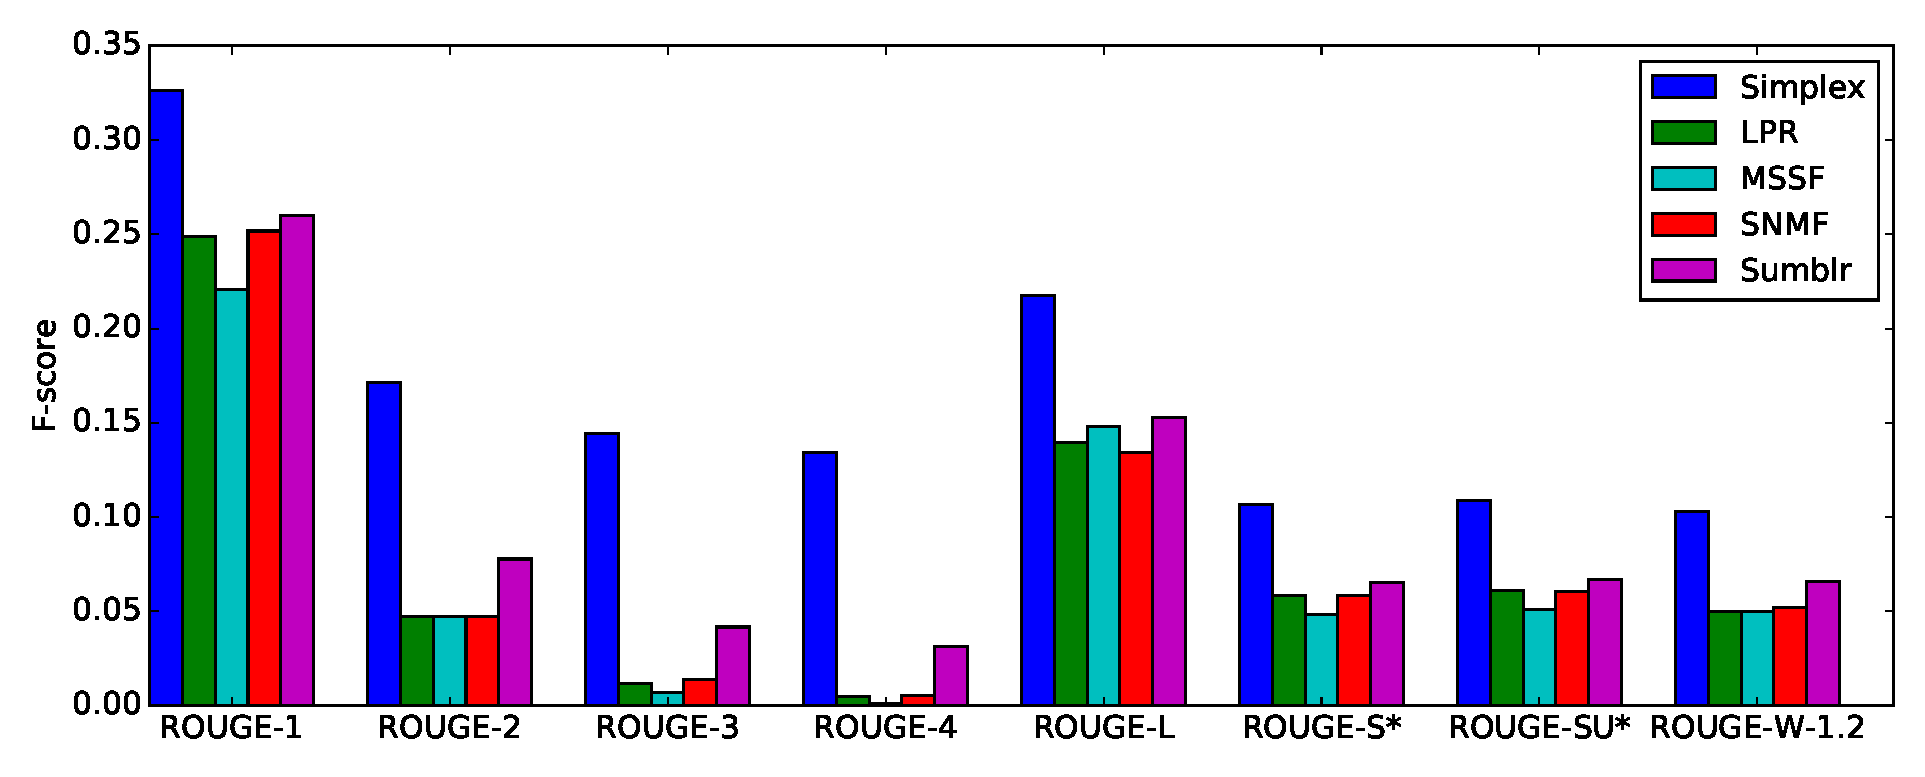
\includegraphics[width=\textwidth]{rouge.eps}
\caption{Average ROUGE F-score on 10 events by different methods.}
\end{figure}



\subsection{Inconsistency Detection Performance}
%comparative methods
Next we study the integrity of summaries generated by different methods. As events in our dataset vary in the length of their lifespan, we select the first 4 timesegments for every event, and compute the inconsistent rate of the summary produced by each method. We first adopt the inconsistency detection strategy in Sec.~\ref{sec:dynamic} to identify inconsistent reports in each summary, and then we manually check the inconsistent reports. We finally obtain the inconsistent rate, which is the proportion of the number of inconsistent reports to the number of reports in a summary.  

As shown in Fig.~\ref{fig:conflictRatio}, the proposed method preserves the integrity of the summary. At each time segment, the median, 25th and 75 percentile of the inconsistent rate over all event summaries produced by the proposed methods are all near zero. On the contrary, the state-of-the-art comparative methods can not generate an consistent summary. LPR and SNMF are better than MSSF and Sumblr, possibly due to the fact that LPR and SNMF tend to select a smaller number of reports. Sumblr and MSSF tend to select more redundant reports, thus the possibility of inconsistency is increased.
%result table or figure
\begin{figure}\label{fig:conflictRatio}
    \centering
    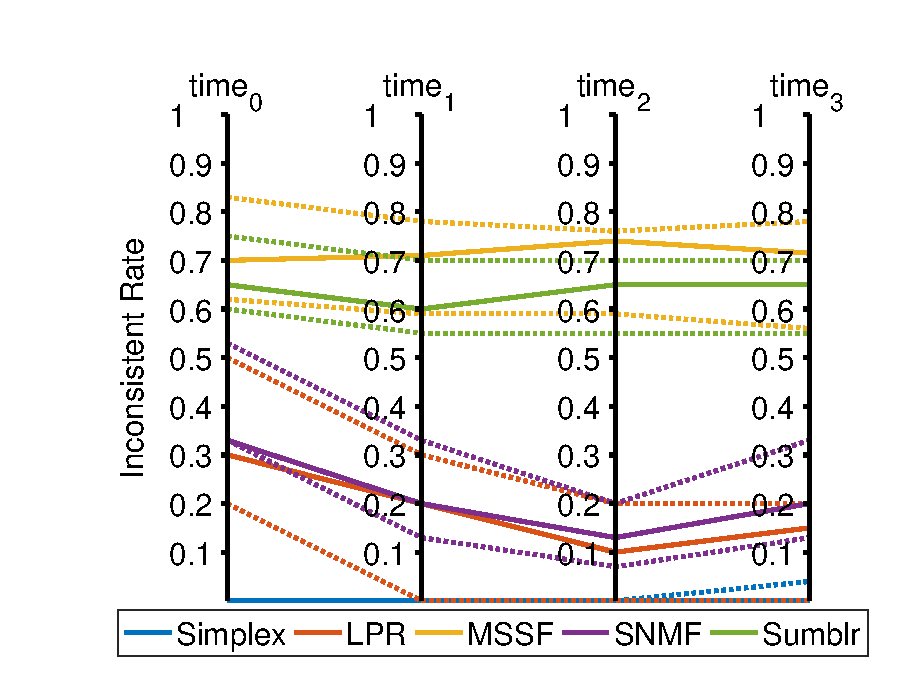
\includegraphics[width=0.8\textwidth]{conflictRatio.eps}
    \caption{Inconsistent rate, including median (solid line), the  25th percentile and the 75th percentile (dashed line) over ten events on first four time segments for each method .}
\end{figure}

\subsection{Efficiency Study}

%goal
%Operating system
We now analyze the effciency of the various techniques. We implemented the proposed algorithm in java and use the open source code for LPR,MSSF, SNMF and Sumblr. All comparative methods are given the set of candidates in each time segment. All experiments have been executed on a server with an Intel(R) Xeon(R) CPU E5-1660 3.20G Hz (4 cores)and main memory 64G bytes.


%result figure
As some methods adopt incremental updating (i.e. Sumblr and ours) while some do not (i.e. LPR,MSSF,SNMF), efficiency analysis must be seperated for the first summary and the summaries afterwards. We report execution times of each method in generating summary in the first time segment, averaged over all events in Fig.~\ref{fig:time0}. The graph y-axes have logarithmic scale to illustrate the difference more clear. We can see that the proposed algorithm is the fastest. We emphasize here that the proposed algorithm is 10 times faster than the second fast method Sumblr, which is also an incremental updating summarization system.  This highlights the potential of our proposed method, since generating realtime summaries is critical during distaster events. 

 We then report the average excution times by different methods, over all events and all follow-up time segments in Fig.~\ref{fig:time1}. We see that again our proposed method is the fastest. Compared with Fig.~\ref{fig:time0}, the excution times for LPR,MSSF and SNMF to generate follow-up summaries differ by two orders of magnitude. This is expected as LPR,MSSF and SNMF are not incremental methods. Thus they are not suitable for delivering real-time summaries. However, Sumblr and our proposed method are more efficient in updating the summaries, as recomputation is limited to a small range of reports.   
\begin{figure}
  \centering
\subfigure[First time segment]{\label{fig:time0}
    \centering
    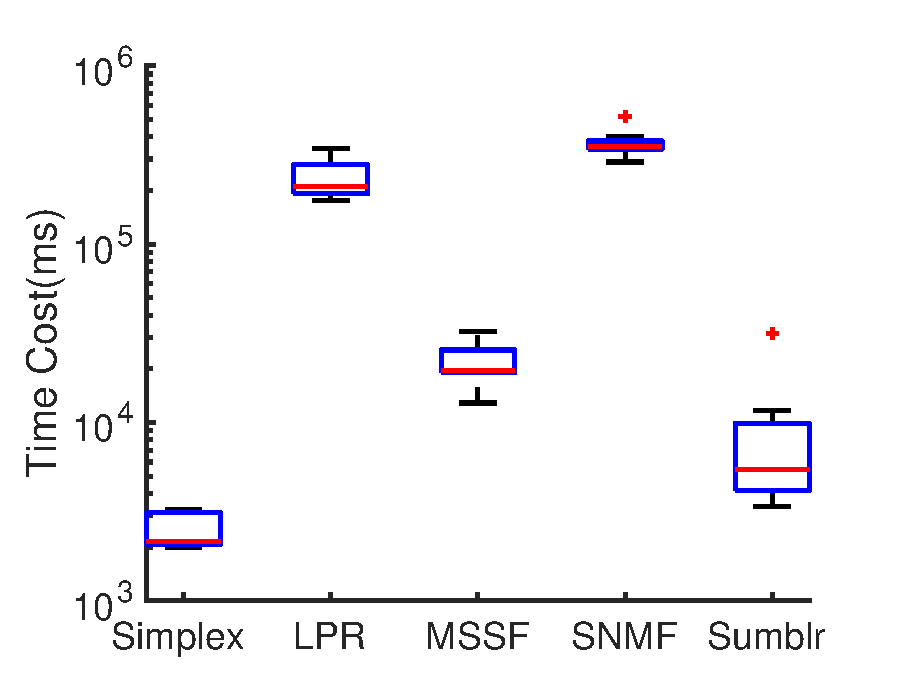
\includegraphics[width =.4\textwidth]{time0.eps}
}
\hspace{-6ex}
\subfigure[Follow-up time segments ]{\label{fig:time1}
    \centering
    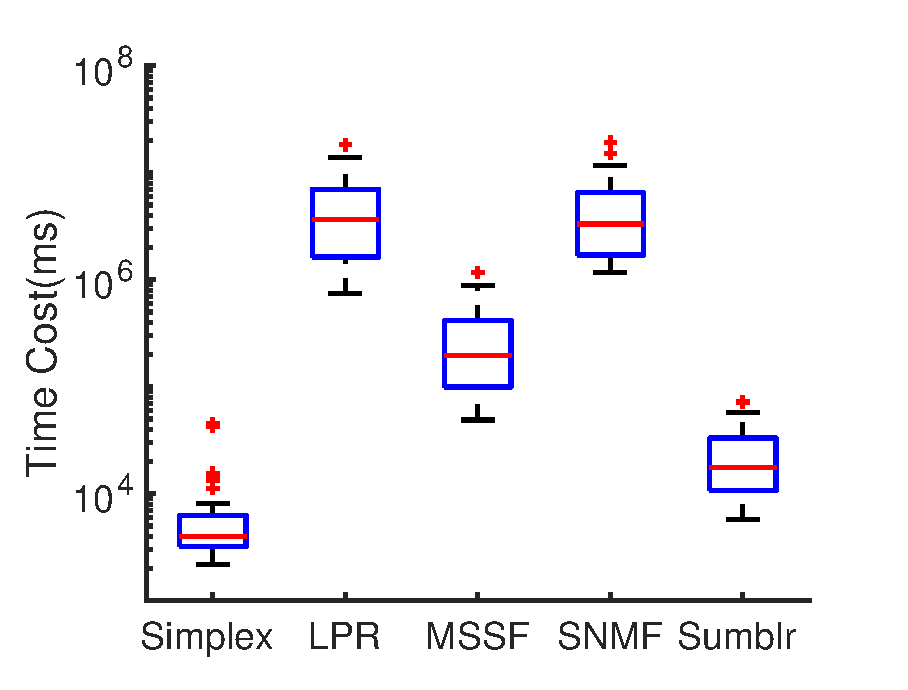
\includegraphics[width =.4\textwidth]{time1.eps}
}
\caption{Average excutation times to generate a summary by various methods. }
\end{figure}

\subsection{Effects of Parameters}

%goal
Finally we examine the effects of parameters in the efficiency of the proposed method. We study the effect of the size of credible and relevant tweets (the number of seeds $M$ in Sec.~\ref{sec:static}) in Fig.~\ref{fig:summary}. The excution time is the time cost to generate the first summary. We set $M=\{50,100,150,200,250,300\}$. We can see that the excution time grows linearly with the size of credible and relevant tweet. However when the number of seeds is too big, the time cost is significantly higher. We observe similar patterns in Fig.~\ref{fig:window}, where the reported excution time is averaged  over all time segments for each event. The time cost grows linearly with the size of time segment when the time window is small. However when the time window is too wide, the time cost is significantly higher. The above too observations suggest that in order to generate realtime summary, it is better to segment the timeline into more divisions and limit the size of seeds.

%result figure
\begin{figure}
  \centering
\subfigure[$M$]{\label{fig:summary}
  \centering
    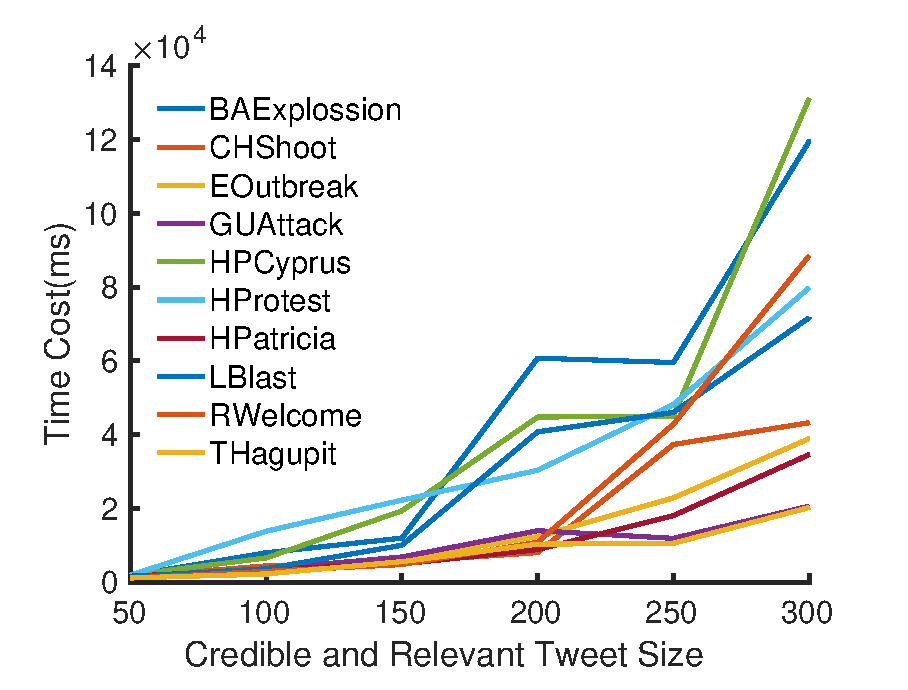
\includegraphics[width =.4\textwidth]{summary.eps}}
\hspace{-6ex}
\subfigure[$T$]{\label{fig:window}
  \centering
    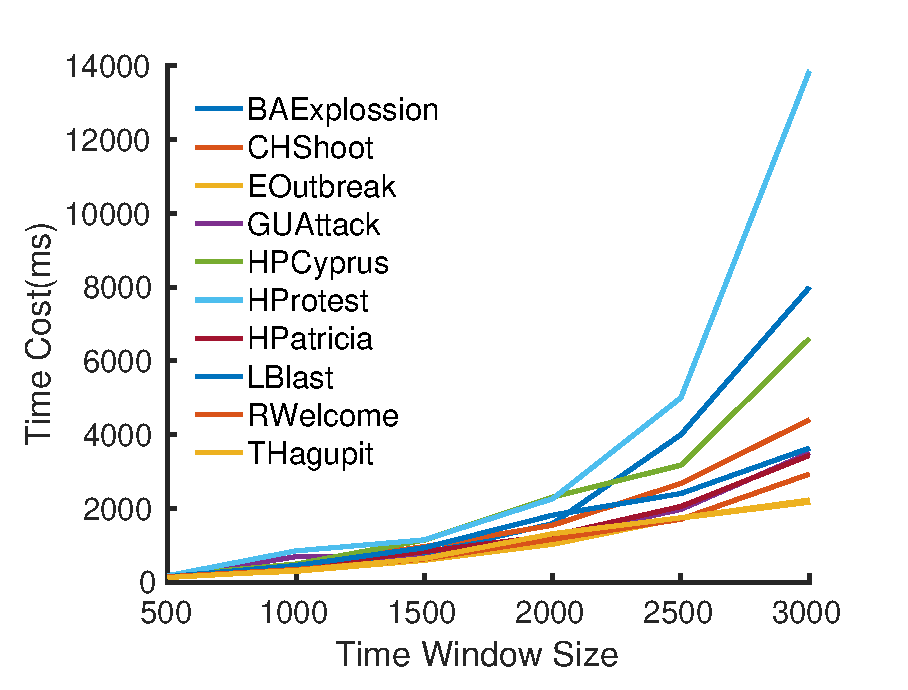
\includegraphics[width =.4\textwidth]{window.eps}
}
\caption{Excution times to generate summary for each event by the proposed method, given different values of parameters.}
\end{figure}

\section{Conclusion}\label{sec:conclusion}
 In this paper we study the problem of realtime event summarization. We implement inconsistency detection in the update procedure to preserve integrity of the summary. We model the realtime summarization problem as integer programming problems and solve the relaxed linear programming form by simplex method. We present a novel inconsistency detection strategy and embed it in the simplex algorithm. Our work shed insights in intellectural information management in social media platforms, and is espetially important for disaster monitoring systems. Our future direction includes exploring more advanced inconsistency detection strategies and exploiting state-of-the-art numerical optimization techniques to solve the integer programming problems. 

\begin{thebibliography}{10}

\bibitem{Chin2017TOTEM}
J.~Y. Chin, S.~S. Bhowmick, and A.~Jatowt.
\newblock Totem: Personal tweets summarization on mobile devices.
\newblock In {\em Proceedings of the 40th International ACM SIGIR Conference on
  Research and Development in Information Retrieval}, SIGIR '17, pages
  1305--1308, New York, NY, USA, 2017. ACM.

\bibitem{Efron2011Estimation}
M.~Efron and G.~Golovchinsky.
\newblock Estimation methods for ranking recent information.
\newblock In {\em Proceedings of the 34th international ACM SIGIR conference on
  Research and development in Information}, SIGIR '11, pages 495--504, New
  York, NY, USA, 2011. ACM.

\bibitem{Gillani2017Post}
M.~Gillani, M.~U. Ilyas, S.~Saleh, J.~S. Alowibdi, N.~Aljohani, and F.~S.
  Alotaibi.
\newblock Post summarization of microblogs of sporting events.
\newblock In {\em Proceedings of the 26th International Conference on World
  Wide Web Companion}, WWW '17 Companion, pages 59--68, Republic and Canton of
  Geneva, Switzerland, 2017. International World Wide Web Conferences Steering
  Committee.

\bibitem{Hannon2010Recommending}
J.~Hannon, M.~Bennett, and B.~Smyth.
\newblock Recommending twitter users to follow using content and collaborative
  filtering approaches.
\newblock In {\em Proceedings of the fourth ACM conference on Recommender
  systems}, RecSys '10, pages 199--206, New York, NY, USA, 2010. ACM.

\bibitem{kwak2010twitter}
H.~Kwak, C.~Lee, H.~Park, and S.~Moon.
\newblock What is twitter, a social network or a news media?
\newblock In {\em Proceedings of the 19th international conference on World
  wide web}, pages 591--600. ACM, 2010.

\bibitem{Lin2012Generating}
C.~Lin, C.~Lin, J.~Li, D.~Wang, Y.~Chen, and T.~Li.
\newblock Generating event storylines from microblogs.
\newblock In {\em Proceedings of the 21st ACM international conference on
  Information and knowledge management}, CIKM '12, pages 175--184, New York,
  NY, USA, 2012. ACM.

\bibitem{Liu2016LEDS}
Z.~Liu, Y.~Huang, and J.~R. Trampier.
\newblock Leds: Local event discovery and summarization from tweets.
\newblock In {\em Proceedings of the 24th ACM SIGSPATIAL International
  Conference on Advances in Geographic Information Systems}, GIS '16, pages
  53:1--53:4, New York, NY, USA, 2016. ACM.

\bibitem{Mathioudakis2010TwitterMonitor}
M.~Mathioudakis and N.~Koudas.
\newblock Twittermonitor: trend detection over the twitter stream.
\newblock In {\em Proceedings of the 2010 international conference on
  Management of data}, SIGMOD '10, pages 1155--1158, New York, NY, USA, 2010.
  ACM.

\bibitem{Meng2012Entitycentric}
X.~Meng, F.~Wei, X.~Liu, M.~Zhou, S.~Li, and H.~Wang.
\newblock Entity-centric topic-oriented opinion summarization in twitter.
\newblock In {\em Proceedings of the 18th ACM SIGKDD international conference
  on Knowledge discovery and data mining}, KDD '12, pages 379--387, New York,
  NY, USA, 2012. ACM.

\bibitem{Ren2013Personalized}
Z.~Ren, S.~Liang, E.~Meij, and M.~de~Rijke.
\newblock Personalized time-aware tweets summarization.
\newblock In {\em Proceedings of the 36th international ACM SIGIR conference on
  Research and development in information retrieval}, SIGIR '13, pages
  513--522, New York, NY, USA, 2013. ACM.

\bibitem{Lin2008Storyline-based}
F.~ren Lin and C.-H. Liang.
\newblock Storyline-based summarization for news topic retrospection.
\newblock {\em Decision Support Systems}, 45(3):473 -- 490, 2008.
\newblock <ce:title>Special Issue Clusters</ce:title>.

\bibitem{Rudra2016Summarizing}
K.~Rudra, S.~Banerjee, N.~Ganguly, P.~Goyal, M.~Imran, and P.~Mitra.
\newblock Summarizing situational tweets in crisis scenario.
\newblock In {\em Proceedings of the 27th ACM Conference on Hypertext and
  Social Media}, HT '16, pages 137--147, New York, NY, USA, 2016. ACM.

\bibitem{Rudra2015Extracting}
K.~Rudra, S.~Ghosh, N.~Ganguly, P.~Goyal, and S.~Ghosh.
\newblock Extracting situational information from microblogs during disaster
  events: A classification-summarization approach.
\newblock In {\em Proceedings of the 24th ACM International on Conference on
  Information and Knowledge Management}, CIKM '15, pages 583--592, New York,
  NY, USA, 2015. ACM.

\bibitem{Sharifi2010Summarizing}
B.~Sharifi, M.-A. Hutton, and J.~Kalita.
\newblock Summarizing microblogs automatically.
\newblock In {\em Human Language Technologies: The 2010 Annual Conference of
  the North American Chapter of the Association for Computational Linguistics},
  HLT '10, pages 685--688, Stroudsburg, PA, USA, 2010. Association for
  Computational Linguistics.

\bibitem{Shou2013Sumblr}
L.~Shou, Z.~Wang, K.~Chen, and G.~Chen.
\newblock Sumblr: continuous summarization of evolving tweet streams.
\newblock In {\em Proceedings of the 36th international ACM SIGIR conference on
  Research and development in information retrieval}, SIGIR '13, pages
  533--542, New York, NY, USA, 2013. ACM.

\bibitem{Takamura2011Summarizing}
H.~Takamura, H.~Yokono, and M.~Okumura.
\newblock Summarizing a document stream.
\newblock In {\em Proceedings of the 33rd European conference on Advances in
  information retrieval}, ECIR'11, pages 177--188, Berlin, Heidelberg, 2011.
  Springer-Verlag.

\bibitem{Wang2009Evolutionary}
D.~Wang, L.~Zheng, T.~Li, and Y.~Deng.
\newblock Evolutionary document summarization for disaster management.
\newblock In {\em Proceedings of the 32nd international ACM SIGIR conference on
  Research and development in information retrieval}, pages 680--681. ACM,
  2009.

\bibitem{Yan2011Evolutionary}
R.~Yan, X.~Wan, J.~Otterbacher, L.~Kong, X.~Li, and Y.~Zhang.
\newblock Evolutionary timeline summarization: a balanced optimization
  framework via iterative substitution.
\newblock In {\em Proceedings of the 34th international ACM SIGIR conference on
  Research and development in Information}, pages 745--754. ACM, 2011.

\bibitem{Yih2007Multi-document}
W.~Yih, J.~Goodman, L.~Vanderwende, and H.~Suzuki.
\newblock Multi-document summarization by maximizing informative content-words.
\newblock In {\em Proceedings of IJCAI}, volume~7, 2007.

\bibitem{Zubiaga2012Towards}
A.~Zubiaga, D.~Spina, E.~Amig\'{o}, and J.~Gonzalo.
\newblock Towards real-time summarization of scheduled events from twitter
  streams.
\newblock In {\em Proceedings of the 23rd ACM conference on Hypertext and
  social media}, HT '12, pages 319--320, New York, NY, USA, 2012. ACM.

\bibitem{ZubiagaTwitterDatasets}
A.~Zubiaga.
\newblock A Longitudinal Assessment of the Persistence of Twitter Datasets.
\newblock In {\em Journal of the Association for Information Science and Technology}.

\bibitem{BloomFilter}
B.~Bloom.
\newblock Space/time tradeoffs in hash coding with allowable errors.
\newblock Communications of the ACM,13(7):422-426,1970.

\bibitem{ROUGE}
C.~Y.~Lin.
\newblock Rouge: A package for automatic evaluation of summaries;
\newblock proceedings of the Text Summarization Branches Out: Proceeding of the ACL-04 workshop, F, 2004[C], Barcelona, Spain.

\bibitem{LPR}
G.~Erkan, D.~R.~Radev.
\newblock LexPageRank: Prestige in Multi-Document Text Summarization.
\newblock In {\em Conference on Empirical Methods in Natural Language Processing}, EMNLP 2004, Barcelona, Spain. DBLP, 2004:365-371.

\bibitem{MSSF}
J.~X.~Li, L.~Li, T.~Li.
\newblock MSSF: A Multi-Document Summarization Framework based on Submodularity.
\newblock  In {\em Proceedings of the 34th international ACM SIGIR conference on Research and development in Information retrieval},SIGIR '11, pages 1247--1248, New York, NY, USA, 2011. ACM.

\bibitem{SNMF}
D.~Wang, T.~Li, S.~Zhu ,D.~Chris.
\newblock Multi-document summarization via sentence-level semantic analysis and symmetric matrix factorization.
\newblock In {\em Proceedings of the 31th international ACM SIGIR conference on
  Research and development in information retrieval}, SIGIR '08, pages
  307--314, Singapore, 2008. ACM.

\bibitem{Finkel2005Incorporating}
Jenny Rose Finkel, Trond Grenager, and Christopher Manning.
\newblock Incorporating Non-local Information into Information Extraction Systems by Gibbs Sampling. 
\newblock In {\em Proceedings of the 43nd Annual Meeting of the Association for Computational Linguistics}, ACL 2005, pp. 363-370. 

\end{thebibliography}


\end{document}
